
\documentclass{llncs}
\usepackage{graphicx}        % standard LaTeX graphics tool
                             % when including figure files
\usepackage{url}
%%%%%%%%%%%%%%%%%%%%%%%%%%%%%%%%%%%%%%%%%%%%%%%%%%%%%%%%%%%%%%%%%%%%%%%%%%%%%%%%%%%%%%%%%
\usepackage{subfigure}
\begin{document}
\sloppy

\title{Increasing User Engagement in a Volunteer-Based Ephemeral Evolutionary Computation System}
\titlerunning{Increasing User Engagement in Volunteer Evolutionary Computing}


\author{Mario Garc\'ia-Valdez\inst{1} \and Juan J. Merelo Guerv\'os\inst{2} \and  Lucero Lara \inst{1}}

\institute{Instituto Tecnol\'ogico de Tijuana, Tijuana BC, Mexico
\and
Universidad de Granada, Granada, Spain
\email{mario@tectijuana.edu.mx}\\
\email{jmerelo@geneura.ugr.es}}

\authorrunning{Garc\'ia-Valdez, Merelo, \& Lara }

\maketitle


\begin{abstract}

One way of creating distributed computing system is to use volunteers who
provide their own computing resources or storage to contribute to a common effort.
By runnning a script in a web page, collaboration is straightforward, but also ephemeral.
Resources depend on the amount of time a user lends, whicn means that 
the user has to be kept engaged to obtain as many computing cycles as
possible. In this paper, we analyze a volunteer-based evolutionary computing system called
NodIO with the objective of discovering rules that encourage volunteer
participation thus increasing the overall computing power. We present the results of
an experiment where a gammification technique is applied by adding a leaderboard 
showing the top scores achieved by registered contributors. In the NodIO system volunteers can
participate without the need to create an account, so the question was
if the need to register would have a negative impact on user participation. 
The experiment results show that even if only a small percentege of users created an account,
those participating in the competition provided around 90\%.

\keywords{Distributed Evolutionary Algorithms, Volunteer Computing}
\end{abstract}

\section{Introduction}

The World Wide Web provides not only a platform for content
distribution, but also, thanks to the maturity and reliability of the
HTTP protocol, an increasingly reliable and high-performance
operating system for running distributed applications. Besides the
protocol itself, there are two factors that contribute to this fact:
the JavaScript virtual machine every browser runs \cite{paulson2005building}
and the simplified standard interface for interacting with servers
exemplified by the REST application interface convention \cite{masse2011rest}.
Thus creating a distributed computing experiment is just a matter of
making a JavaScript application interchange information with a server,
by using REST. From the point of view of the programmer, this involves
relatively common skills and no special libraries, since the
interface is built in the browser, and a simple application that
responds to those requests on the server side; both involve just a few
dozens lines of code additionally to whatever business logic the
application has. But, more importantly and from the point of view of
the user, that application can be run by simply visiting a web page.

Using this approach for creating distributed experiments is called {\em
  volunteer}, {\em cycle-scavenging}, or {\em opportunistic} computing
\cite{sarmenta2001volunteer} and it dates back, in different shapes
and underlying mechanisms, to the origin of the web \cite{david-seti:home}. Our interest
here, however, is to use it as a resource for evolutionary
computation, as our group has done for a long time \cite{jj-ppsn98}.

In this line of research that uses volunteer computing for
evolutionary algorithms, there are several pending issues. The first
and maybe most important is approaching volunteer computing as a
socio-technical system \cite{vespignani2009predicting} which integrates
user decisions and behavioral patterns in the system model; this
includes trying to optimize the number of users in a particular
experiment. The second line of research, although related to the
first, is more focused on the evolutionary algorithm itself and how
different design decisions will affect its performance.
% Is it ok that we say that the first line of research is the most important... but then we focus on the second?
We have approached the first issue in our previous work \cite{jj-ppsn98},
% I have justified to focus, in this case, on the second
but in this paper our focus will be in the second aspect: we will try to
design a decentralized system that, at the same time, is able to use
all available resources for finding the solution of an evolutionary algorithm. This design will be done incrementally by
changing client and the server and measuring its
impact on the overall performance: time and evaluations needed to find
the solution. Eventually, we want to find a system that, whatever the
number of users available to perform the experiment, is able to
maximize their contribution to the evolutionary algorithm, at the same
time that the evolutionary algorithm itself makes the most of those
contributions and is able to find
the solution to the problem in a minimum time, with the least
number of contributions.

The rest of the paper is organized as follows: Next we will briefly
present the state of the art in opportunistic distributed evolutionary
computation (EC). Section \ref{sec:description} will describe the
framework and problem used in the experiments, which are publicly
available under a free license. We will present the results of the
different steps in the incremental design in Section
\ref{sec:experiments}, to finally wrap up with the conclusions.

\begin{figure*}[t]
    \centering
        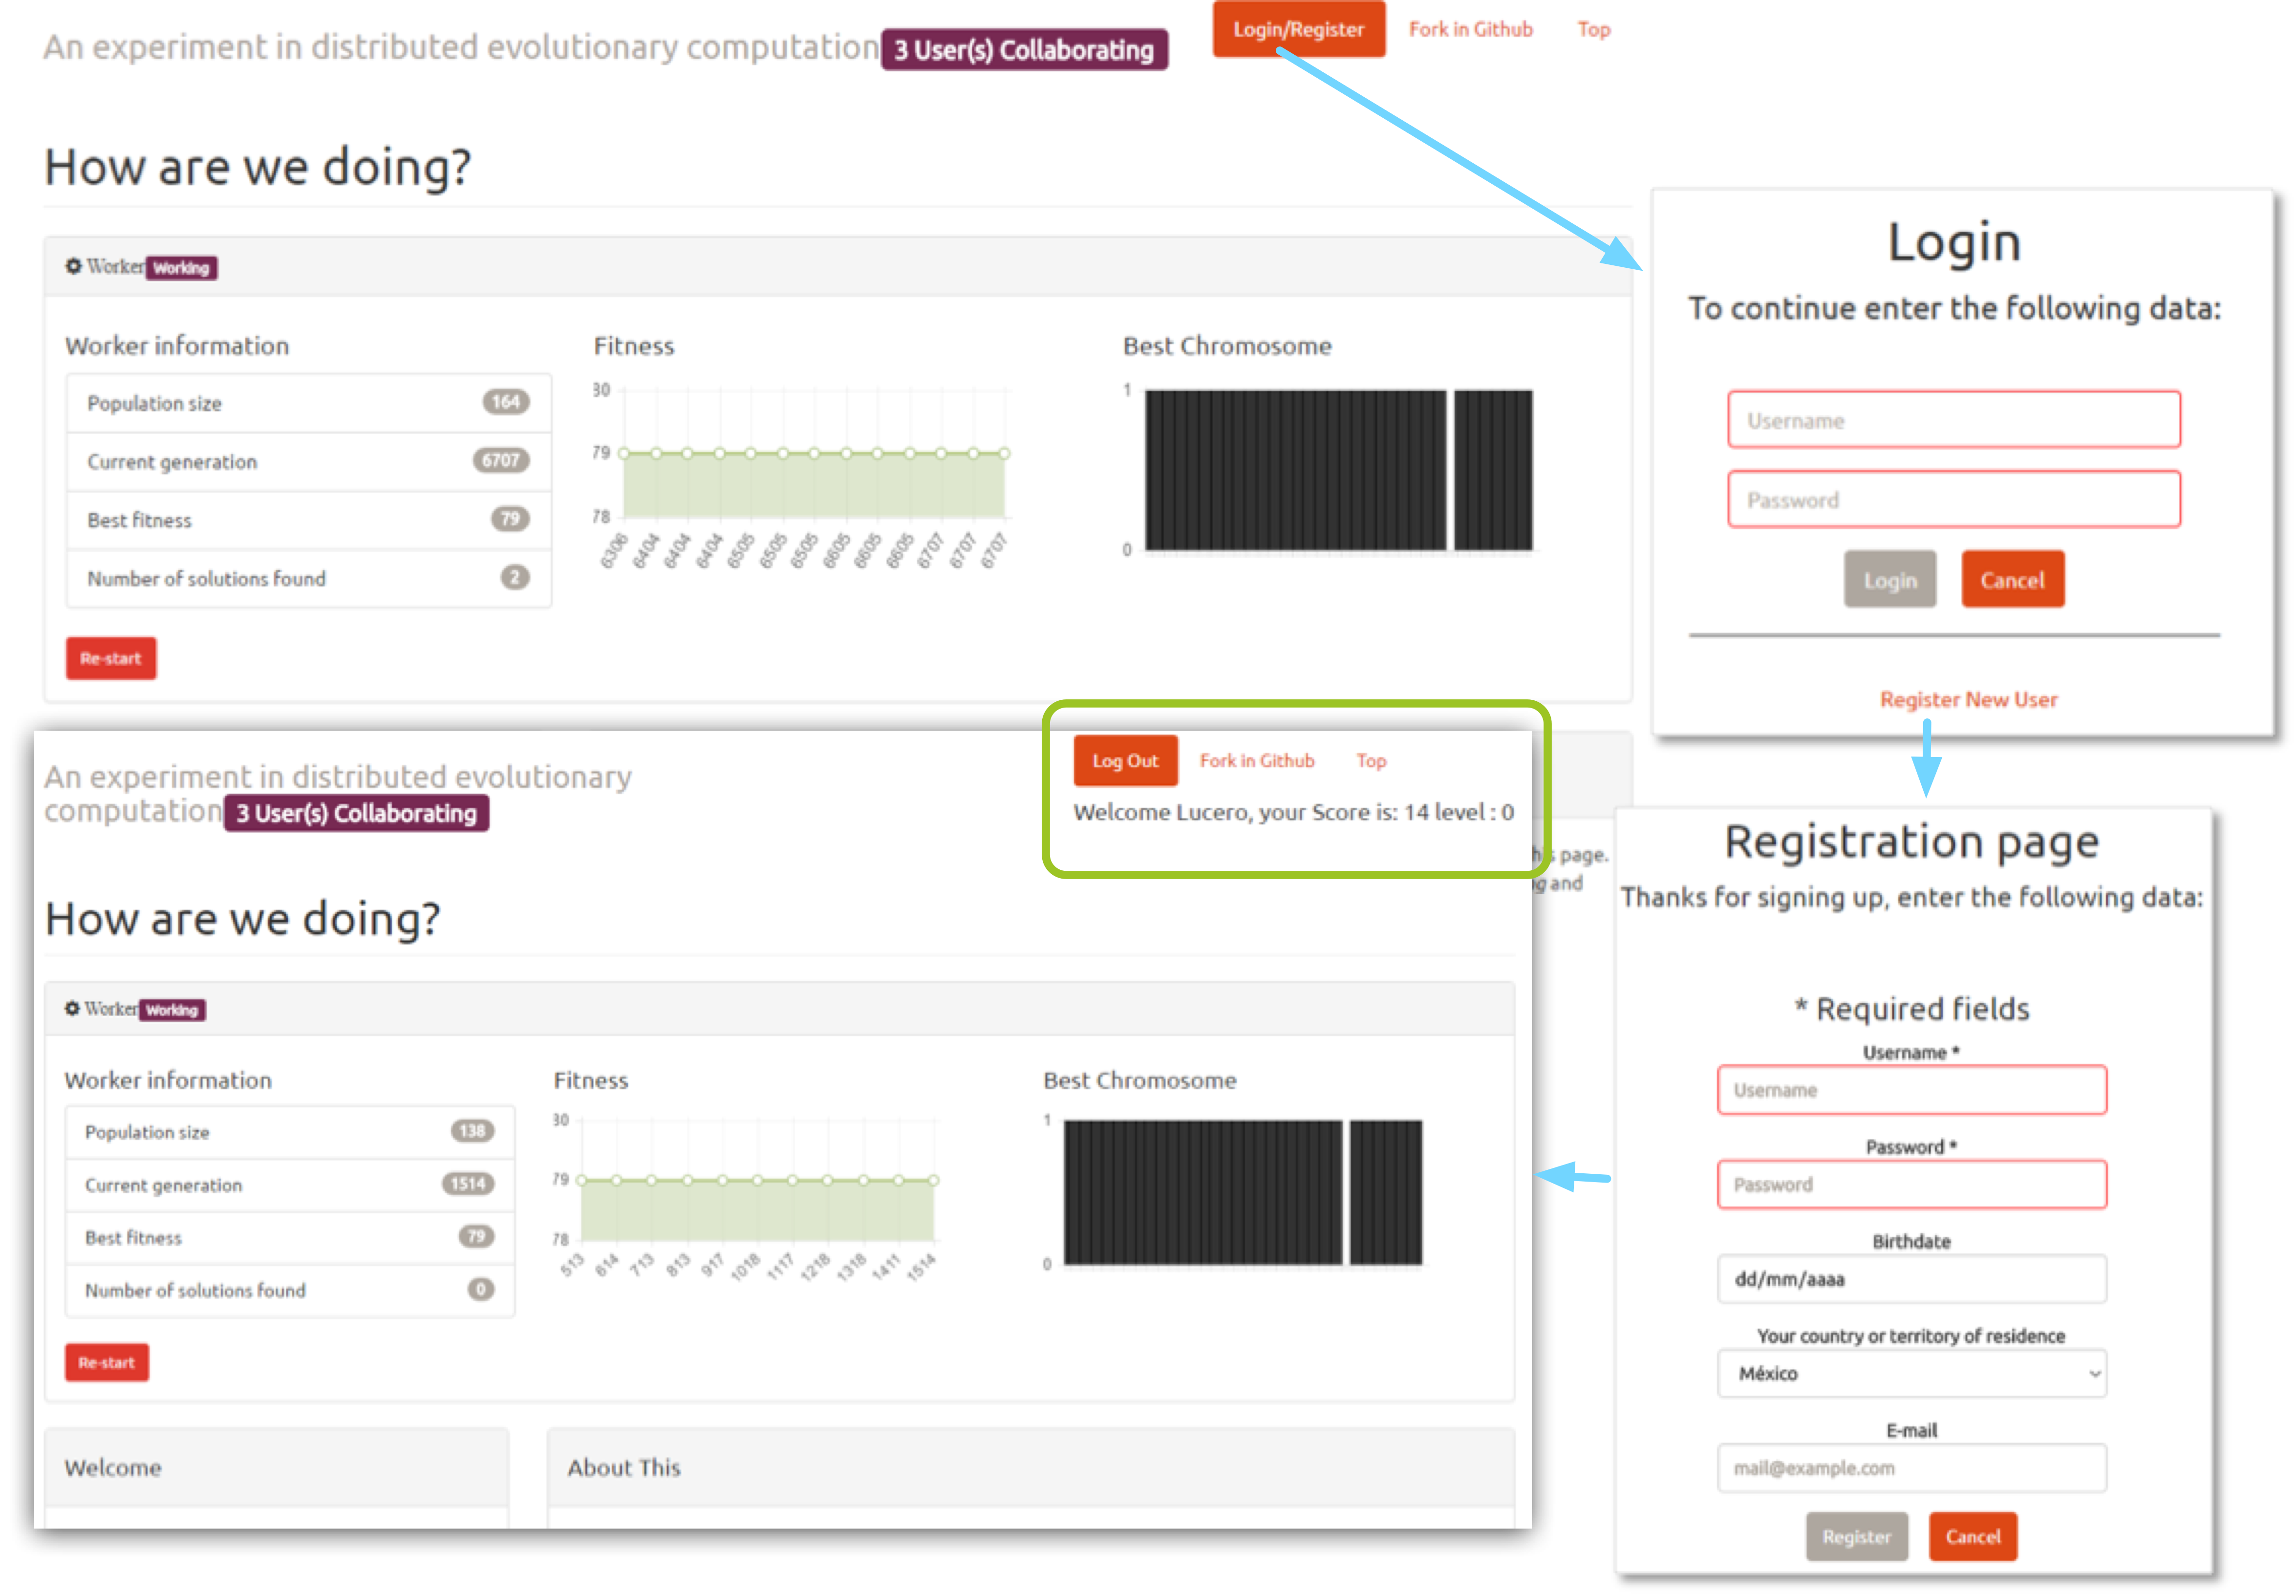
\includegraphics[width=5in]{img/login.png}
    \caption{Comparison of 30 runs of the 128 Bit OneMax problem. 
    Box-plot of the number of evaluations needed for solution, with a 2, 6 and 12 workers
    homogeneous configuration on the left side, and Heterogeneous configuration on the
    right side of each.
    }
    \label{fig:comp-onemax}
\end{figure*}

\section{Experiments}
\label{sec:experiments}

\subsection{Results}
\label{sec:results}

\begin{figure*}[t]
    \centering
    \subfigure  [6 workers]
    {
        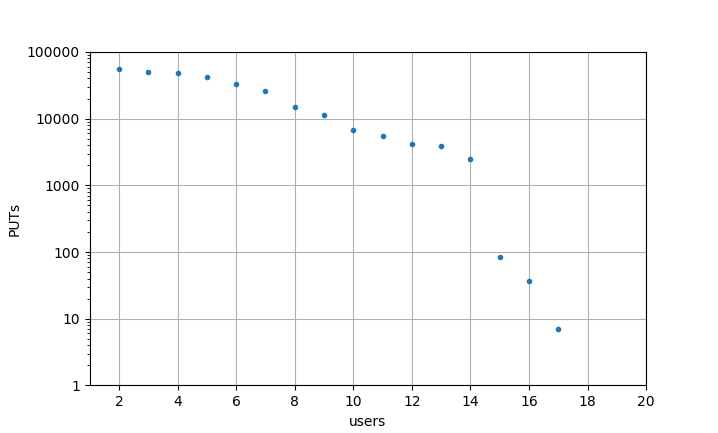
\includegraphics[width=4in]{img/puts_user.png}
    }
    \subfigure  [12 workers]
    {
        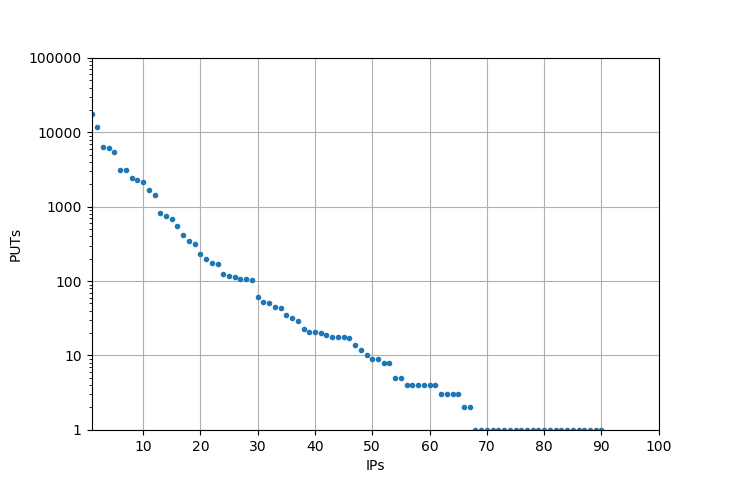
\includegraphics[width=4in]{img/puts_ip.png}
    }

    \caption{100 experiments with random parameters for the 128 Bit Griewank 
    single-objective optimization test function. Experiments are ranked by 
    the mean time to solution of 5 runs, with (a) 6 workers, and (b) 12 workers.}
    \label{fig:griewank}
\end{figure*}


\begin{figure*}[t]
    \centering
        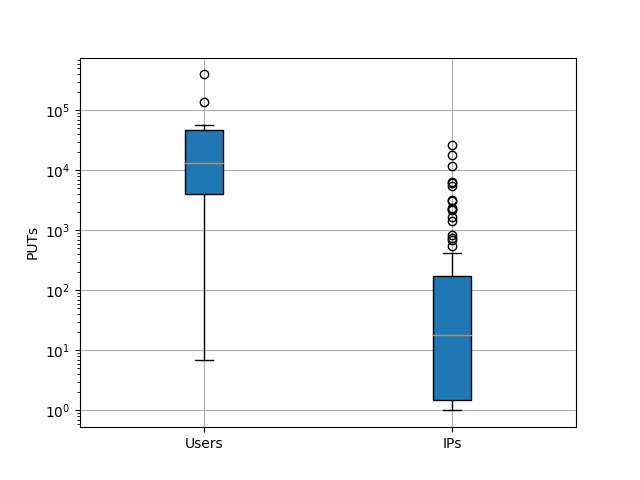
\includegraphics[width=4in]{img/puts_box.png}
    \caption{Comparison of 30 runs of the 128 Bit OneMax problem. 
    Box-plot of the number of evaluations needed for solution, with a 2, 6 and 12 workers
    homogeneous configuration on the left side, and Heterogeneous configuration on the
    right side of each.
    }
    \label{fig:comp-onemax}
\end{figure*}

\begin{figure*}[t]
    \centering
        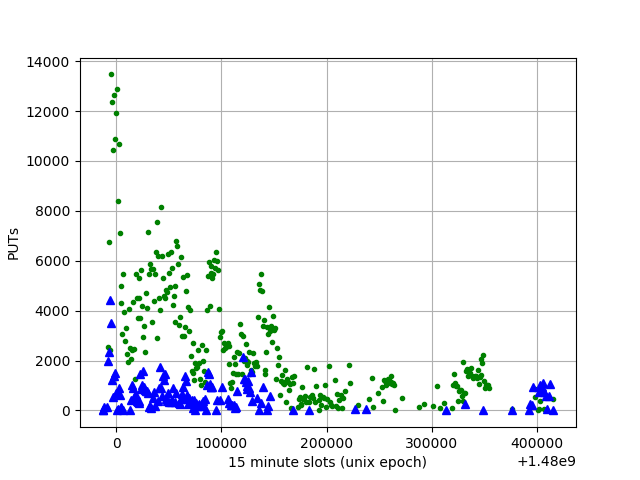
\includegraphics[width=5in]{img/puts_by_time.png}
    \caption{Comparison of 30 runs of the 128 Bit OneMax problem. 
    Box-plot of the number of evaluations needed for solution, with a 2, 6 and 12 workers
    homogeneous configuration on the left side, and Heterogeneous configuration on the
    right side of each.
    }
    \label{fig:comp-onemax}
\end{figure*}
\begin{figure*}[t]
    \centering
        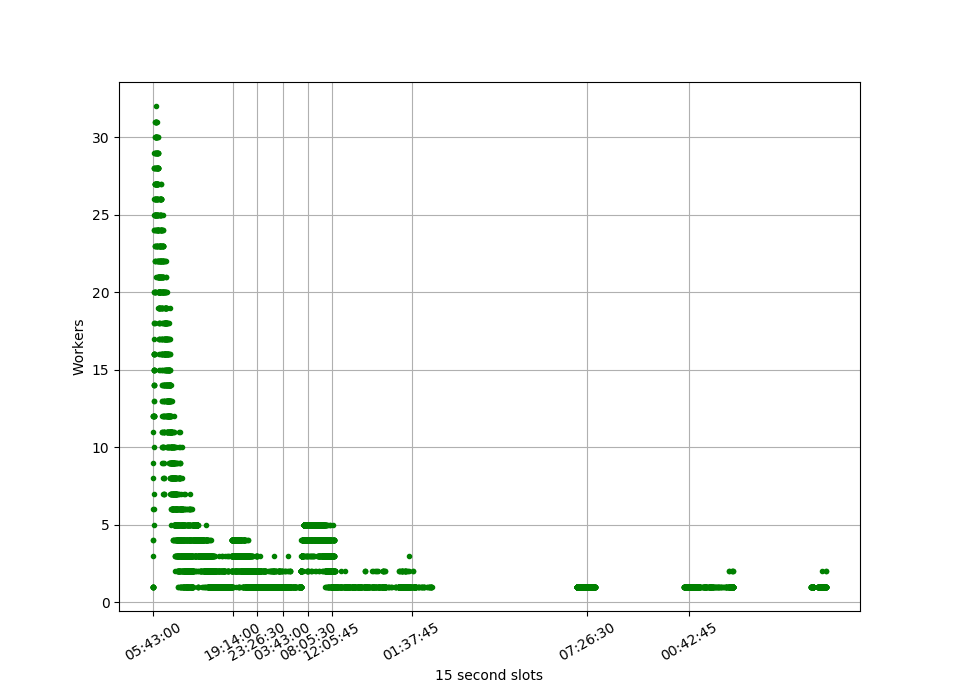
\includegraphics[width=5in]{img/workers_best_user.png}
    \caption{Comparison of 30 runs of the 128 Bit OneMax problem. 
    Box-plot of the number of evaluations needed for solution, with a 2, 6 and 12 workers
    homogeneous configuration on the left side, and Heterogeneous configuration on the
    right side of each.
    }
    \label{fig:comp-onemax}
\end{figure*}
\begin{figure*}[t]
    \centering
        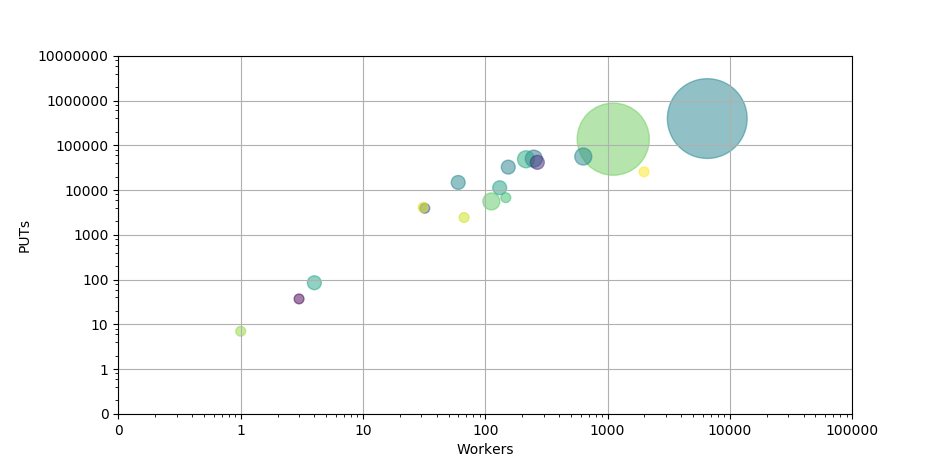
\includegraphics[width=5in]{img/workers_put_ip.png}
    \caption{Comparison of 30 runs of the 128 Bit OneMax problem. 
    Box-plot of the number of evaluations needed for solution, with a 2, 6 and 12 workers
    homogeneous configuration on the left side, and Heterogeneous configuration on the
    right side of each.
    }
    \label{fig:comp-onemax}
\end{figure*}

\bibliographystyle{splncs03}
\bibliography{volunteer,GA-general,geneura,javascript,ror-js}
\end{document}
